% !TEX program = xelatex
\documentclass[oneside,letterpaper,14pt]{memoir} 
\usepackage{graphicx} % Required for inserting images
\usepackage{fontspec} % For custom fonts with XeLaTeX/LuaLaTeX
\usepackage[hidelinks]{hyperref}
\usepackage{setspace}
\usepackage{pdfpages}
\pageletter
\usepackage{geometry}
\usepackage[spanish]{babel}

\geometry{
  left=1.0in,
  right=1.0in,
  top=1in,
  bottom=1in
}

\chapterstyle{section}

% Load your custom fonts
\setmainfont{ArnoPro-Regular.ttf}[
  Path = ./fonts/,
  BoldFont = ArnoPro-Bold.ttf,
  ItalicFont = ArnoPro-Italic.ttf,
  BoldItalicFont = ArnoPro-BoldItalic.ttf
]

\newfontfamily\teutonic[Path=./fonts/]{Teutonic.ttf}

% Set chapter and section fonts
\setsecheadstyle{\teutonic\Large\bfseries}
\setsubsecheadstyle{\teutonic\large\bfseries}
\setsubsubsecheadstyle{\teutonic\normalsize\bfseries}

% Set chapter style
\renewcommand{\chaptitlefont}{\teutonic\Huge\bfseries}
\renewcommand{\chapnumfont}{\teutonic\Huge\bfseries}

\title{The Haunting}
\author{Edgar M. Miranda}
\date{\today}

% Title formatting
\pretitle{\begin{center}\teutonic\Huge\bfseries}
\posttitle{\end{center}}
\preauthor{\begin{center}\Large}
\postauthor{\end{center}}
\predate{\begin{center}\large}
\postdate{\end{center}}

\begin{document}
\maketitle

\frontmatter
% \chapter{Dedication}
% \chapter{Copyright}
% \chapter{Acknowledgements}

% \maxtocdepth{subsection}
\tableofcontents

% \listoffigures
% \listoftables

% \part{The first part}

\mainmatter


% \setsecnumdepth{subsection} % use numbers for subsection

% Handouts
\chapter{Handout 1}

\emph{Un propietario, el señor Knott, le pide que examine una casa antigua en el
centro de Boston, conocida como la Casa Corbitt. Los antiguos inquilinos, la
familia Macario, se vieron envueltos en una tragedia y el dueño desea entender
los misteriosos sucesos de la casa y aclarar el asunto. El señor Knott no ha
podido alquilar la casa desde la tragedia y espera que usted pueda aclarar las
cosas y restaurar su buen nombre. Se ofrece a pagarle por su tiempo y sus
molestias, a razón de \$20 al día. El propietario le da las llaves, la dirección
y \$20  en efectivo por adelantado.}

\emph{Dada la naturaleza de su trabajo, usted querrá realizar algo de
investigación antes de dirigirse a la casa. Podría consultar antiguos artículos
de periódico en las oficinas del \emph{Boston Globe}, dirigirse a la
\emph{Central Library} o ir al \emph{The Hall of Records}. La elección es suya.}

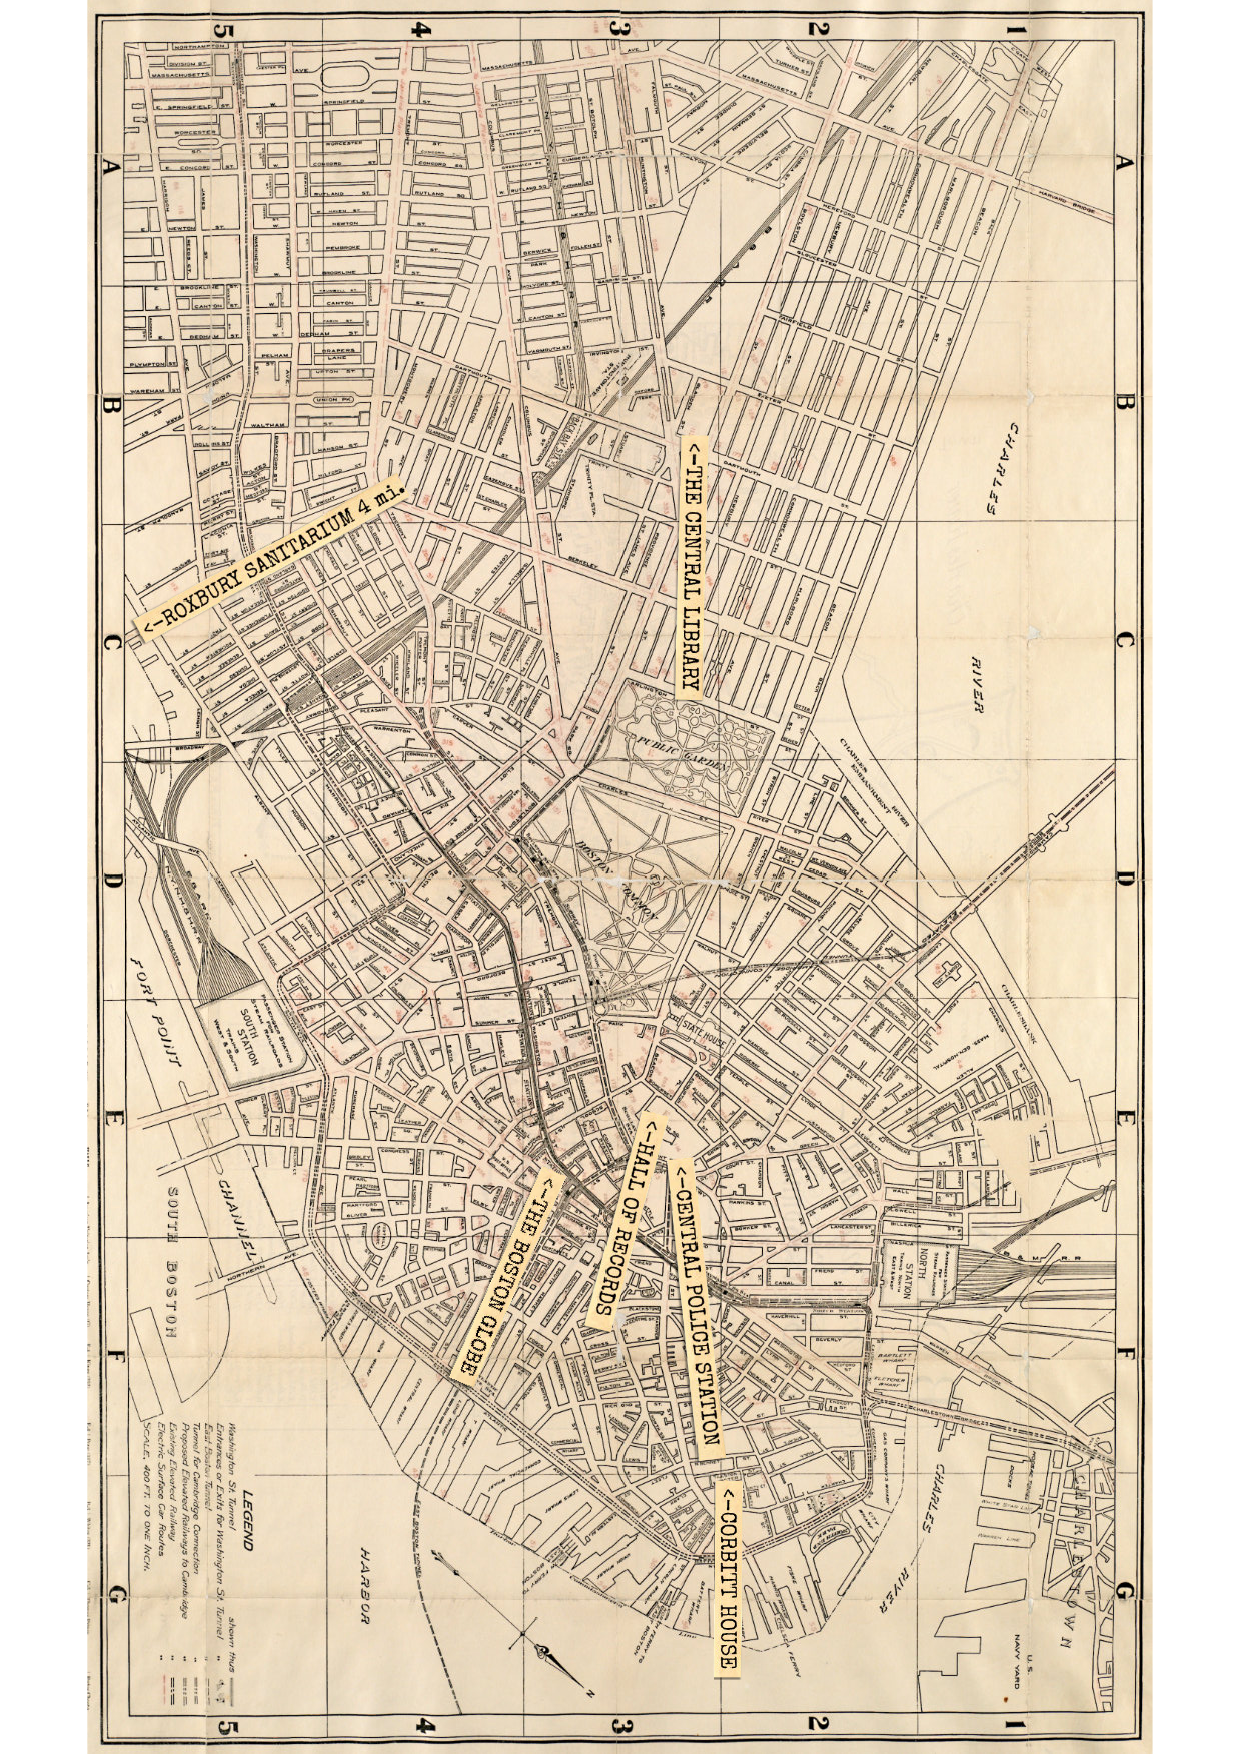
\includepdf[pages={1}, scale=1.0]{./assets/Boston-map.pdf}
\chapter{Handout 2}

\emph{Artículo rechazado del \emph{Boston Globe (1918)} que cuenta sucesos
relacionados a las extrañas tragedias de la casa Corbitt a través de los años}

\includepdf[pages={2}, scale=1.0]{./assets/Unpublished-Story-Boston-Globe-1918.pdf}
\chapter{Handout 3}

\emph{En 1835, un próspero comerciante construye la casa, pero inmediatamente
cae enfermo y se la vende al señor Walter Corbitt, caballero.}

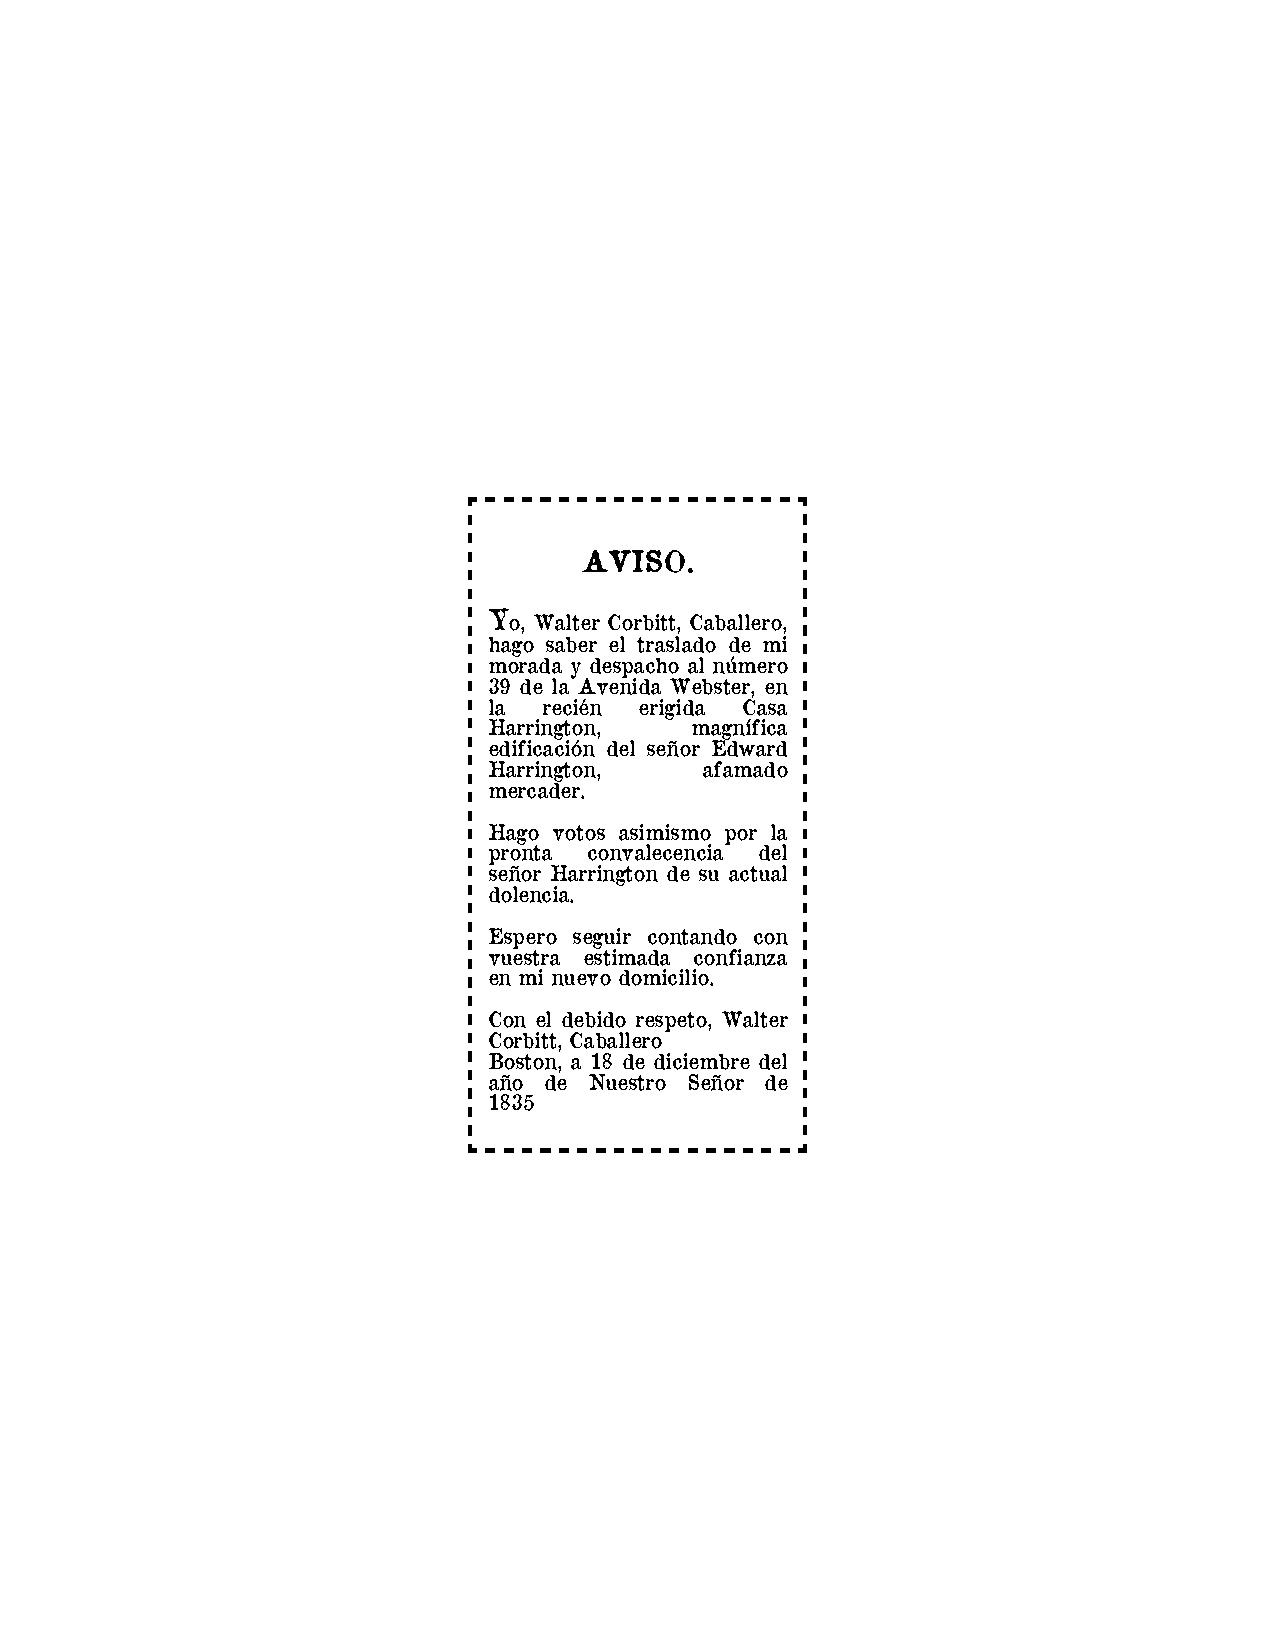
\includepdf[pages={1}, scale=1.0]{./assets/Boston-Globe-Clippings-1835.pdf}
\chapter{Handout 4}

\emph{En 1852, Walter Corbitt es demandado por sus vecinos, quienes presentan
una petición para obligarlo a abandonar la zona “a consecuencia de sus hábitos
sospechosos y su comportamiento poco propicia.}

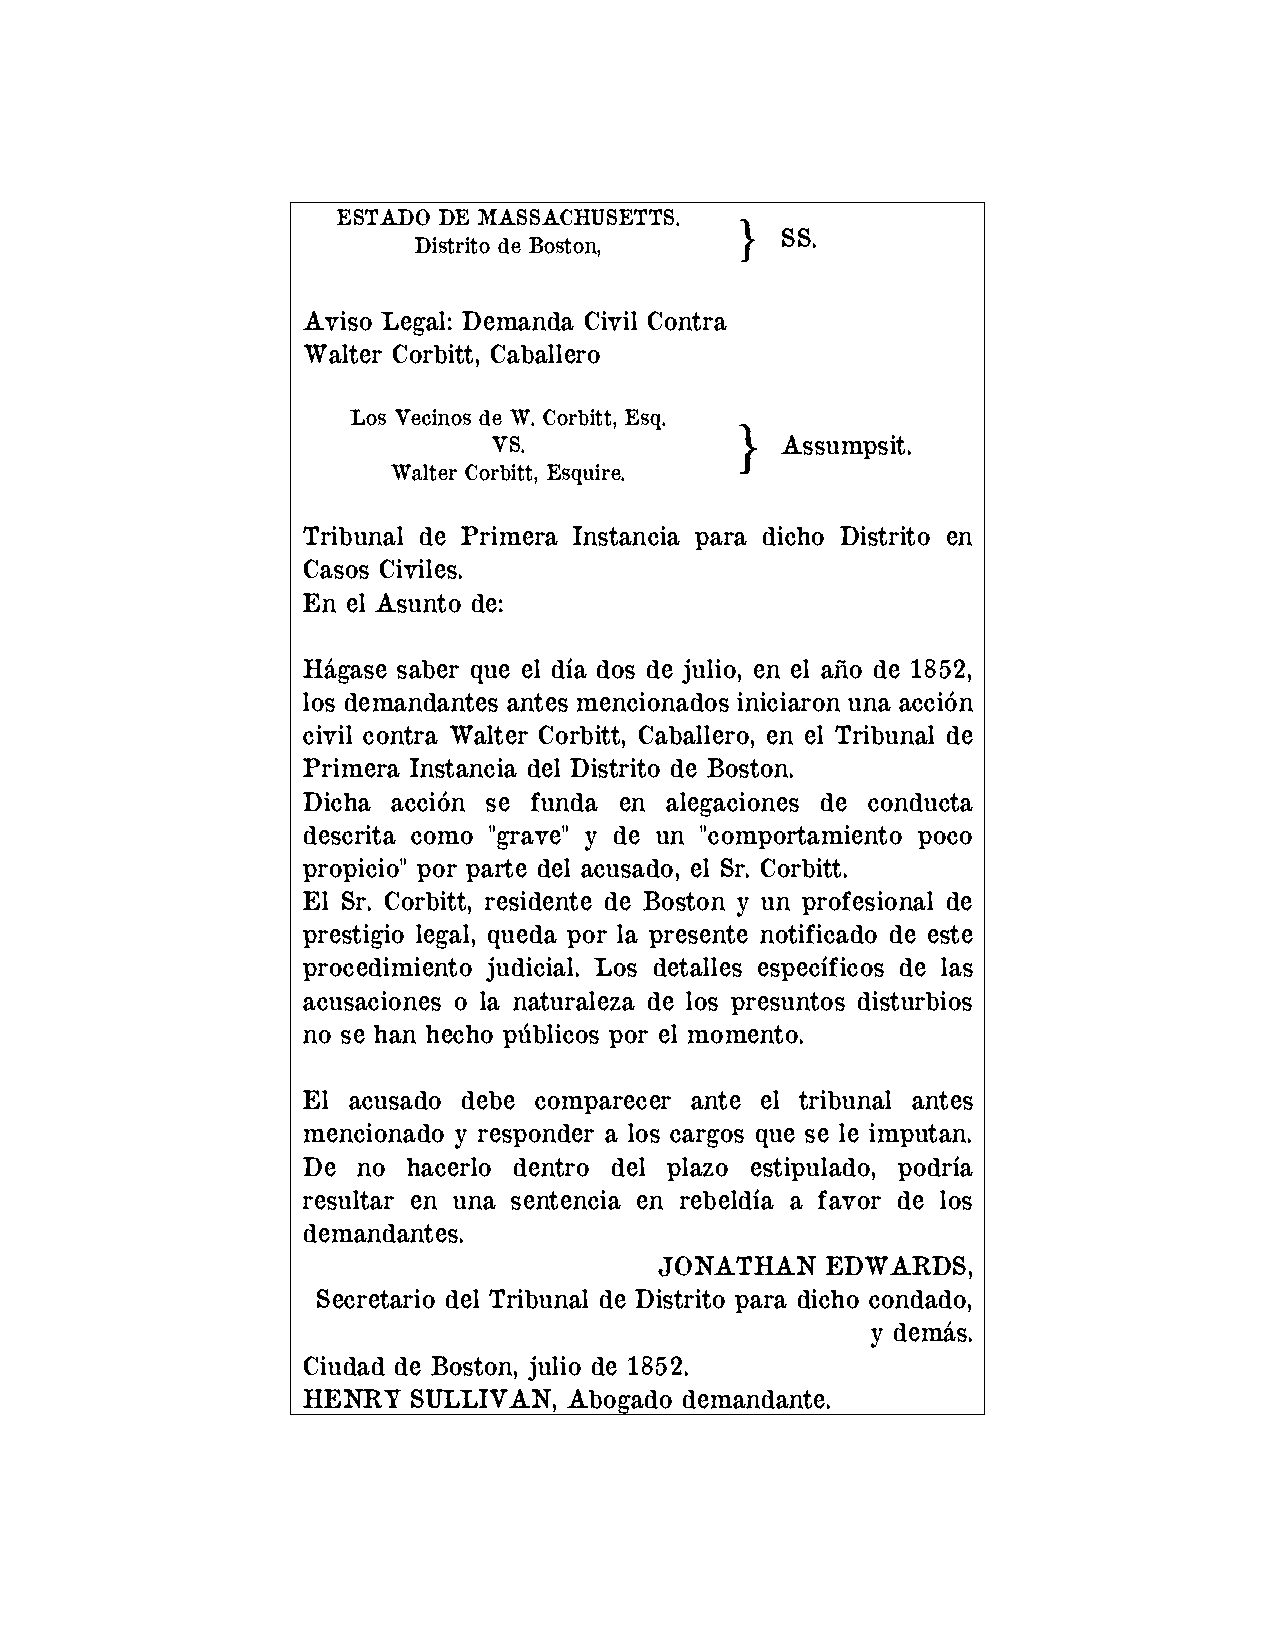
\includepdf[pages={1}, scale=1.0]{./assets/Boston-Globe-Clippings-1852.pdf}
\chapter{Handout 5}

\emph{Evidentemente, Corbitt gana la demanda. Su obituario, publicado en 1866,
indica que aún vivía en el mismo lugar. También menciona que se estaba llevando
a cabo una segunda demanda para impedir que Corbitt fuera enterrado en el sótano
de su casa, tal como lo estipulaba su testamento.}

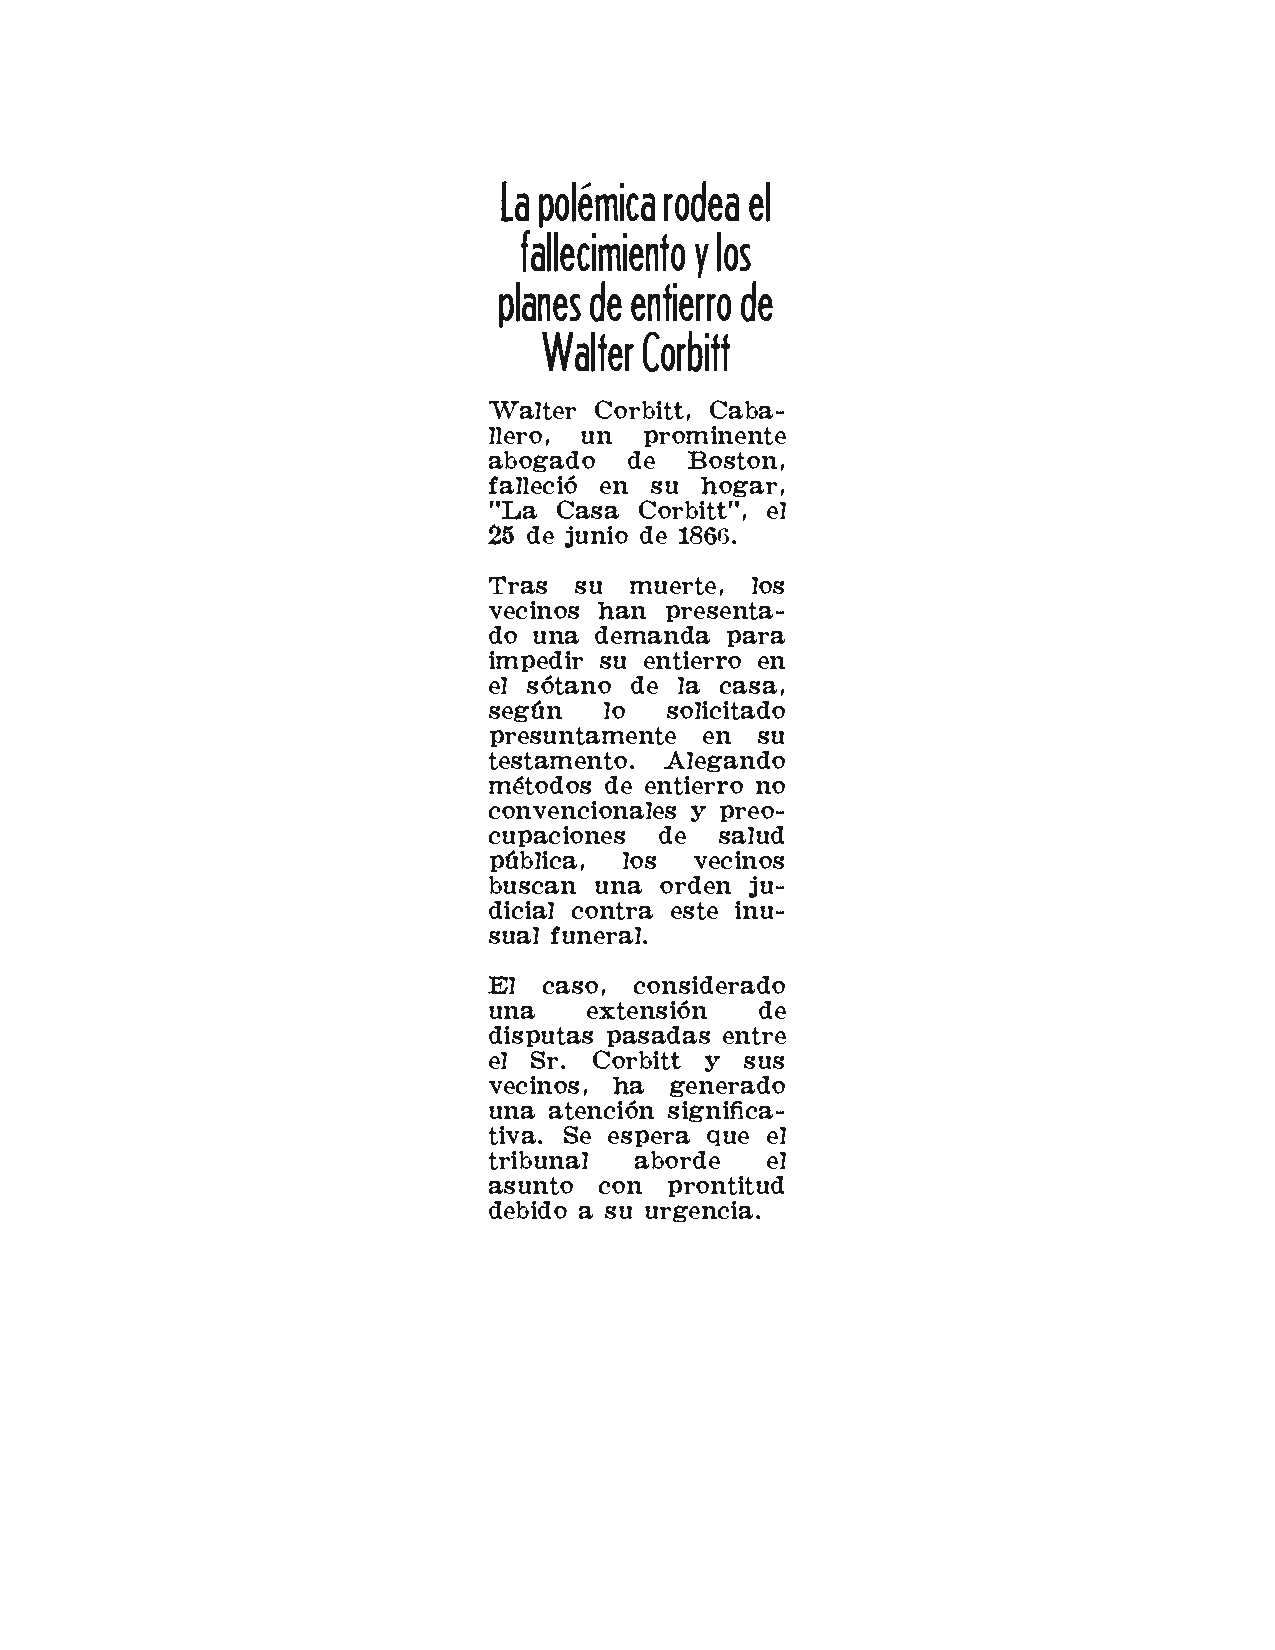
\includepdf[pages={1}, scale=1.0]{./assets/Boston-Globe-Clippings-1866.pdf}
\chapter{Handout 6}

\emph{ No se registra el resultado de la segunda demanda.}
\chapter{Handout 7}

\emph{Los registros del tribunal civil muestran que el albacea del testamento de
Walter Corbitt fue el Reverendo Michael Thomas, pastor de la \emph{Chapel of
Contemplation and Church of Our Lord Granter of Secrets}.}


\includepdf[pages={1}, scale=1.0]{./assets/Sucesion-de-Walter-Corbitt.pdf}

\includepdf[pages={1}, scale=1.0]{./assets/City-of-Boston-Hall-of-Records-chapel-closure.pdf}
\chapter{Handout 8}

\emph{El documento describe una redada secreta en la \emph{Chapel of
Contemplation}. La operación policial fue impulsada por declaraciones juradas
que acusaban a miembros de la iglesia de estar implicados en la desaparición de
niños del vecindario. Durante la redada, murieron tres policías y diecisiete
miembros de la secta, ya sea por disparos o por el fuego. Los informes forenses
resultan inusualmente vagos y poco detallados, como si el forense no hubiera
llevado a cabo los exámenes adecuados.}

\emph{Aunque fueron arrestados 54 miembros de la iglesia, todos menos ocho
fueron liberados. Los registros sugieren que un alto funcionario local
intervino de manera ilegal en el proceso judicial, y que se relataron versiones
de la redada —la mayor operación criminal en la historia de la ciudad— que
jamás llegaron a publicarse.}

\emph{El pastor Michael Thomas fue detenido y condenado a 40 años de prisión
por cinco cargos de asesinato en segundo grado. Sin embargo, escapó de prisión
en 1917 y huyó del estado.}

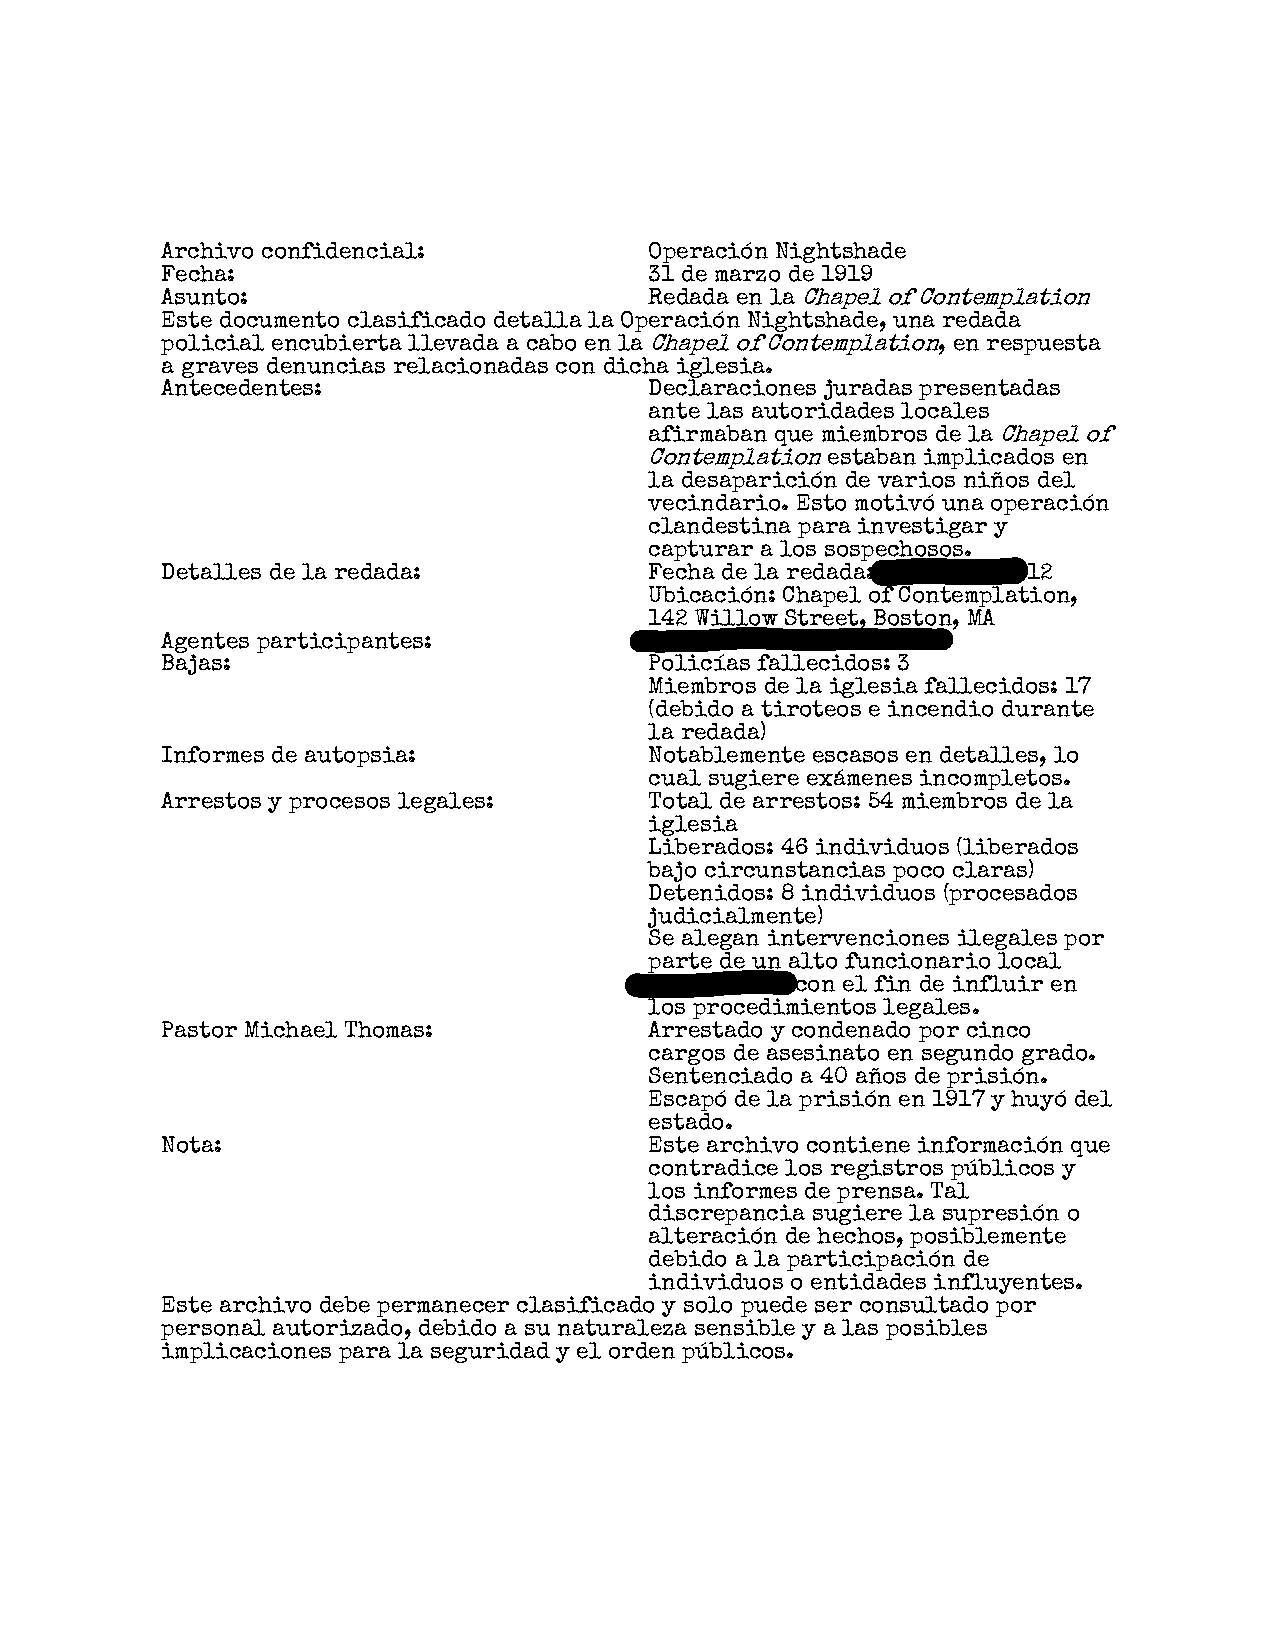
\includepdf[pages={1}, scale=1.0]{./assets/Archivo-confidencial-Operacion-Nightshade.pdf}
\chapter{Handout 9}

\emph{Lo que queda de la vieja iglesia se alza al final de una calle torcida y
lúgubre. Las ruinas están tan desgastadas y cubiertas de vegetación que los
escombros de piedra gris parecen más una roca natural que antiguos muros y
cimientos. Pasas junto a un muro desplomado que ostenta símbolos pintados de
blanco, aparentemente recién trazados: tres letras Y dispuestas en un triángulo
de tal manera que los elementos superiores de cada Y tocan a las otras dos. En
el centro, así creado, está pintado un ojo que mira fijamente.}

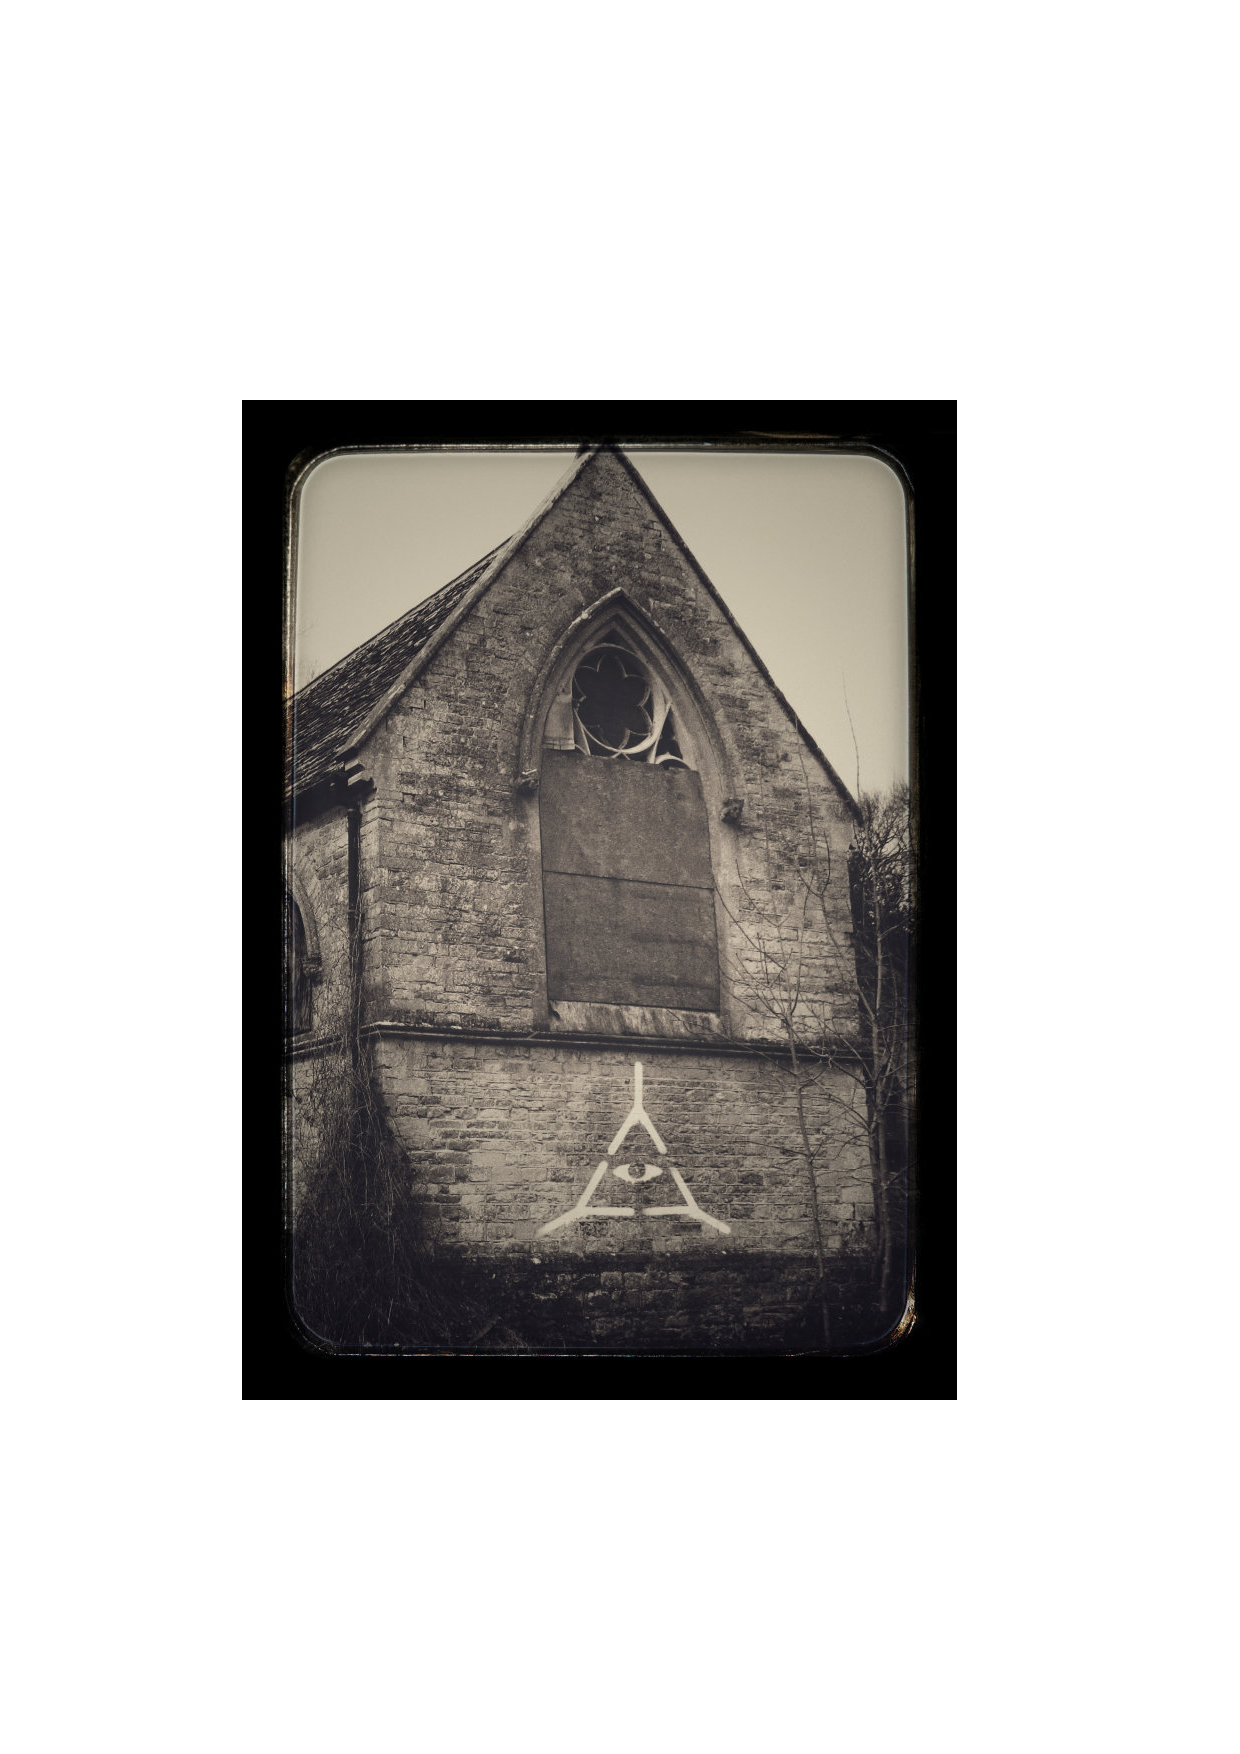
\includepdf[pages={1}, scale=1.0]{./assets/Chapel-symbol.pdf}

\chapter{Descripción de Lugares}

\section{Café} 

Entras al café y, por un momento, el bullicio de la ciudad queda atrás.
El lugar, con su decoración de madera oscura y sus lámparas redondas que
cuelgan del techo como faroles de gas, parece suspendido en el tiempo. Todo en
él (los bancos de cuero gastado, la larga barra de mármol, los espejos
empañados por el humo del tabaco) sugiere que este sitio ha visto más de lo que
deja entrever.

Algunos clientes conversan en voz baja, otros beben solos, absortos en
pensamientos que no comparten. El camarero sirve con precisión mecánica, como
si sus gestos siguieran una coreografía antigua. Detrás de la barra, botellas
alineadas brillan con reflejos apagados, y un reloj que apenas avanza marca una
hora que parece no importar.

El murmullo del lugar se mezcla con el roce de tazas, el tintinear de cucharas
y algún que otro crujido de la madera vieja. Todo tiene un ritmo contenido,
casi expectante, como si este café fuera el escenario silencioso de un misterio
que se cuece lento… y que aún no ha sido revelado.


\section{Boston Globe} 

El Boston Globe, uno de los periódicos más antiguos y de
mayor renombre en la ciudad, con la mayor circulación de toda Nueva Inglaterra,
late con el pulso incesante de las noticias en marcha. El pequeño vestíbulo de
entrada está apenas amueblado y rebosa de movimiento: hombres y mujeres cruzan
de un lado a otro con prisa, llevando papeles, carpetas o simplemente la
urgencia en el rostro.

Más allá, se abre la redacción: una maraña de escritorios de madera golpeada y
archivadores maltrechos, todos tan apretujados que dos personas espalda con
espalda no podrían levantarse sin tropezar. La atmósfera es sofocante, cargada
de humo, tensión y la energía de algo que no se detiene. El ruido es constante:
teléfonos que suenan sin cesar, teclas de máquinas de escribir que repiquetean
como metralla, y voces que se cruzan a gritos, discutiendo titulares, cerrando
ediciones o pidiendo confirmaciones.

No es un lugar cómodo, ni tranquilo, pero aquí, entre el desorden y la presión,
se forjan las historias que llenan las páginas del día siguiente—algunas
verídicas, otras no tanto, pero todas necesarias.

\section{Central Library} 

Entras a la Biblioteca Central en el corazón de Boston. El
edificio, con su imponente arquitectura clásica, transmite una sensación de
solemnidad, como si cada piedra ocultara siglos de historias y secretos. A tu
alrededor, altas estanterías llenas de libros se elevan como murallas
silenciosas, custodiando el conocimiento de generaciones. Al final del amplio
pasillo, el Mostrador de Información se encuentra inmóvil, iluminado por una
luz tenue que parece no alcanzar del todo los rincones del salón. El silencio
es casi absoluto, roto solo por el leve susurro de una página volteada a lo
lejos, un discreto carraspeo o el eco de tus propios pasos sobre el mármol.
Cada sonido resuena con más fuerza de lo esperado, como si el lugar no
estuviera acostumbrado a la presencia humana. Hay algo en el ambiente... una
calma densa, cargada, como si la biblioteca guardara no solo libros, sino
también verdades que no todos deberían descubrir.

\section{Hall of Records} 

La fachada fachada del salón de registros está marcada por numerosas ventanas
en arco, da paso a un interior que replica el mismo lenguaje arquitectónico:
curvas amplias y elegantes que dominan cada puerta y pasillo, como si el lugar
estuviera diseñado para suavizar incluso los asuntos más duros que aquí se
manejan.

Al entrar, te recibe un vestíbulo sobrio pero luminoso. En el centro, un amplio
escritorio preside el espacio, tras el cual una recepcionista sonriente te
observa con cortesía profesional. “Buenas tardes, ¿en qué puedo ayudarle?”,
pregunta con una voz clara y amable. Todo en este lugar sugiere orden,
formalidad… y un archivo bien guardado de todo lo que la ciudad prefiere no
olvidar.

\section{Central Police Station} 

Entras a la comisaría, un sombrío edificio de ladrillo. Su exterior austero no
pretende inspirar confianza, sino imponer autoridad. Al cruzar la puerta, te
recibe un vestíbulo estrecho con olor a papel envejecido, sudor y café
recalentado. Un escritorio desgastado ocupa el centro del espacio, atendido por
un joven oficial de rostro serio y uniforme impecable, que levanta la vista
apenas lo necesario para registrar tu presencia.

Más allá del mostrador, el interior se despliega en filas de escritorios
metálicos y archivadores abollados, cada uno cubierto por pilas desordenadas de
papeles, tazas de café olvidadas y máquinas de escribir que parecen nunca
descansar. El ambiente es ruidoso, tenso, saturado de energía contenida, como
si, en cualquier momento, alguien pudiera irrumpir con noticias urgentes… o con
problemas aún más graves.

\section{The neighborhood}

Lo que alguna vez fue un vecindario apacible y lleno de vida, hoy se percibe
como una sombra de sí mismo. La mayoría de quienes vivían han partido, buscando
mejores oportunidades, otros llevados por el curso natural de los años. Las
pintorescas casas del siglo XIX, con sus porches de madera y jardincillos
descuidados, han desaparecido casi por completo.

En su lugar se alzan ahora edificios de granito y concreto, toscos y
funcionales, al servicio de una economía distinta. Fábricas, talleres mecánicos
y depósitos ocupan las calles donde antes jugaban niños o se escuchaban radios
desde ventanas abiertas. El aire huele a aceite, metal y humo, y hay una
sensación persistente de abandono disfrazado de actividad.
\section{Roxbury Sanitarium}

El Sanatorio de Roxbury fue construido a principios de siglo bajo el nombre de
“Hospital de Tisícos de Boston”, un lugar destinado a que los más pobres de la
ciudad pudieran recuperarse—o al menos morir con dignidad—de la tuberculosis.
Con el tiempo, sin embargo, las prioridades cambiaron. La línea tenue entre la
enfermedad física y el deterioro mental se desdibujó, y cada vez más recursos
del hospital se destinaron al tratamiento de distintas formas de locura.
Finalmente, el sanatorio fue reconvertido en un asilo, uno enteramente dedicado
a contener, tratar y, en muchos casos, simplemente custodiar a los desquiciados
de Boston.

Al entrar, lo primero que ves es un escritorio de recepción, tras el cual una
joven con uniforme blanco inmaculado escribe en un cuaderno de tapas cosidas.
Su caligrafía es meticulosa, su expresión neutra, como si los horrores
cotidianos que la rodean ya no la afectaran.

Una puerta conduce a un pasillo largo, y al caminar por él comienzas a sentir
el peso del lugar. A cada lado, figuras quebradas por la mente se deslizan en
silencio o balbucean en bucles infinitos. Algunos pacientes están sentados en
sillas de ruedas, moviendo las manos en el aire como si intentaran atrapar
cosas que solo ellos pueden ver. Otros vagan tambaleantes, los ojos perdidos,
como ecos de personas que una vez fueron.

\subsection{Versos bíblicos}

\begin{itemize}

    \item \emph{Hay una clase de hombre cuyos dientes son como espadas, y sus
    mandíbulas como cuchillos, hechos para devorar a los afligidos de la faz de
    la tierra. Por su propio instrumento es vencida la sanguijuela.}

    \item \emph{Sed sobrios, velad; porque vuestro adversario el diablo, como
    león rugiente, anda alrededor buscando a quien devorar.}

    \item \emph{Bienaventurado será el que tomare y estrellare a tus pequeñitos
    contra las piedras.}

    \item \emph{Deja que los muertos entierren a sus muertos.}

    \item \emph{No os unáis en yugo desigual con los incrédulos; porque ¿qué
    compañerismo tiene la justicia con la injusticia? ¿Y qué comunión la luz
    con las tinieblas?}

\end{itemize}
\section{The Chapel of Contemplation}

Lo que queda de la vieja capilla se alza al final de un callejón torcido y
sucio que parte desde Sheafe Street, un vestigio de los caminos adoquinados que
alguna vez pisaron severos milicianos y casacas rojas desesperadas. El tiempo
ha sido cruel con la estructura: apenas un esqueleto de lo que fue, devorado
por la intemperie y el olvido.

Los muros restantes están cubiertos por limo rugoso y escamoso que se arrastran
como dedos antiguos sobre la piedra. En las bases, espinas negras de hollín
ascienden en líneas irregulares, como cicatrices dejadas por un fuego que no
consumió del todo, pero sí marcó para siempre. El lugar exhala un aire de
abandono denso, donde el silencio no es quietud, sino espera. Aquí, cada grieta
parece contar una historia perdida… o advertir que no todas han terminado.

\section{The Old Corbitt Place}

Aquí se alza una casa, solitaria, con una arquitectura Federal envejecida que
recuerda los primeros suspiros de la nación. Es una reliquia de otra época,
sentada con obstinación en medio de un vecindario ahora dominado por lo
comercial, como si el tiempo la hubiese rodeado, pero no logrado desalojar.
Taciturna y ensimismada, permanece en penumbra bajo la sombra de estructuras
más nuevas y arrogantes que la flanquean.

La fachada gris verdosa mira hacia la calle con una quietud que incomoda. En la
parte trasera, un jardín descuidado se ahoga bajo maleza espesa, y un emparrado
medio derrumbado apunta al abandono progresivo. Al contemplar la casa, puedes
evitar notar cómo parece replegarse sobre sí misma, deslizándose hacia las
sombras como algo que prefiere no ser visto. Las ventanas, ocultas tras
cortinas pesadas, parecen aferrarse a sus secretos con una fuerza casi física,
como si temieran que, al ceder un poco, algo muy antiguo y muy oscuro pudiera
escapar.


\end{document}
